
En el presente apartado, se realiza un examen detallado de las diversas alternativas tecnológicas y arquitectónicas disponibles que satisfacen los requisitos previamente establecidos para el proyecto. 

Este análisis implica una evaluación rigurosa de las ventajas y desventajas asociadas a cada opción. La finalidad es identificar la solución más apropiada que no solo cumpla con los requisitos funcionales y no funcionales del proyecto, sino que también se alinee óptimamente con las restricciones y objetivos globales del mismo.

\subsubsection{Valoración de alternativas para la arquitectura}
A continuación, se presenta una comparación de varias alternativas arquitectónicas para el desarrollo del sistema.
\subsubsubsection{Arquitectura Monolítica}
La arquitectura monolítica es un enfoque de desarrollo de software en el que una aplicación se construye como una sola unidad. En este caso, todos los componentes del sistema se diseñan y se implementan como un único bloque, que se ejecuta como un único proceso.
Este enfoque en un proyecto pequeño puede ser beneficioso, ya que simplifica el proceso de desarrollo y sobretodo de despliegue. Sin embargo, a medida que el proyecto crece, la arquitectura monolítica se vuelve cada vez más compleja y difícil de mantener. Además, la escalabilidad de la aplicación se ve limitada por la necesidad de escalar el sistema en su conjunto, en lugar de poder escalar componentes individuales de forma independiente.
\begin{figure}[H]
    \centering
    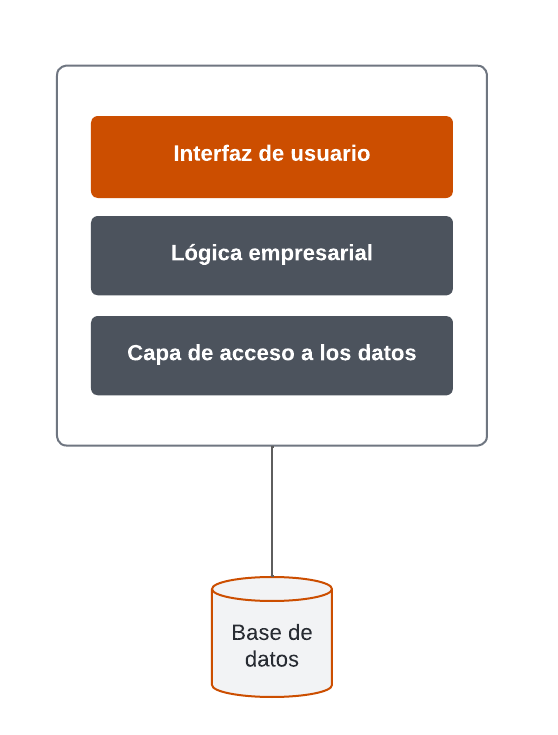
\includegraphics[width=0.4\textwidth]{figures/4-Estudio-viabilidad/4_Monolitica.png}
    \caption{Arquitectura Monolítica}
    \label{fig:arquitectura_monolitica}
    \hypertarget{fig:arquitectura_monolitica}{}
\end{figure}

\subsubsubsection{Arquitectura de Microservicios}
La arquitectura de microservicios es un enfoque de desarrollo de software en el que una aplicación se construye como un conjunto de servicios pequeños, independientes y altamente escalables. Cada servicio se ejecuta como un proceso separado y se comunica con otros servicios mediante mecanismos ligeros, como una API REST.
Este enfoque permite que los servicios se desarrollen, desplieguen y escalen de forma independiente, lo que facilita la gestión de proyectos complejos. Sin embargo, la arquitectura de microservicios también introduce una mayor complejidad en el desarrollo y la gestión de la aplicación, ya que requiere la implementación de mecanismos de comunicación entre los servicios, así como la gestión de la escalabilidad de cada uno de ellos.
\begin{figure}[H]
    \centering
    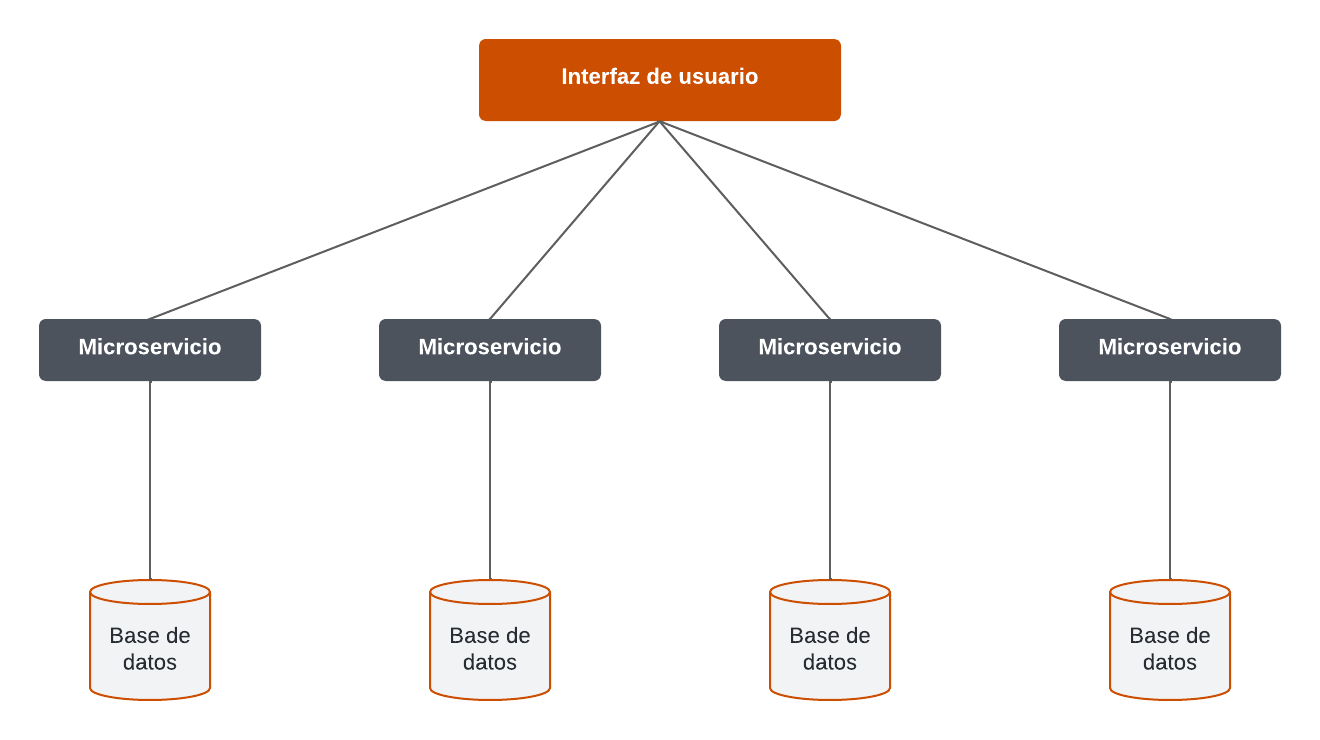
\includegraphics[width=0.7\textwidth]{figures/4-Estudio-viabilidad/4_Microservicios.png}
    \caption{Arquitectura de Microservicios}
    \label{fig:arquitectura_microservicios}
    \hypertarget{fig:arquitectura_microservicios}{}
\end{figure}

\subsubsubsection{Arquitectura de REST API y WepApp}    
Se caracteriza por una clara división entre cliente y servidor, encapsulados respectivamente en WepApp (frontend) y REST API (backend). Esta separación promueve una organización modular, facilitando el mantenimiento del proyecto al separar de forma clara las distintas responsabilidades. 
Este enfoque es un punto intermedio entre las dos arquitecturas anteriores, ya que permite una mayor flexibilidad en el desarrollo y la gestión de la aplicación, sin introducir una complejidad excesiva. 
\begin{figure}[H]
    \centering
    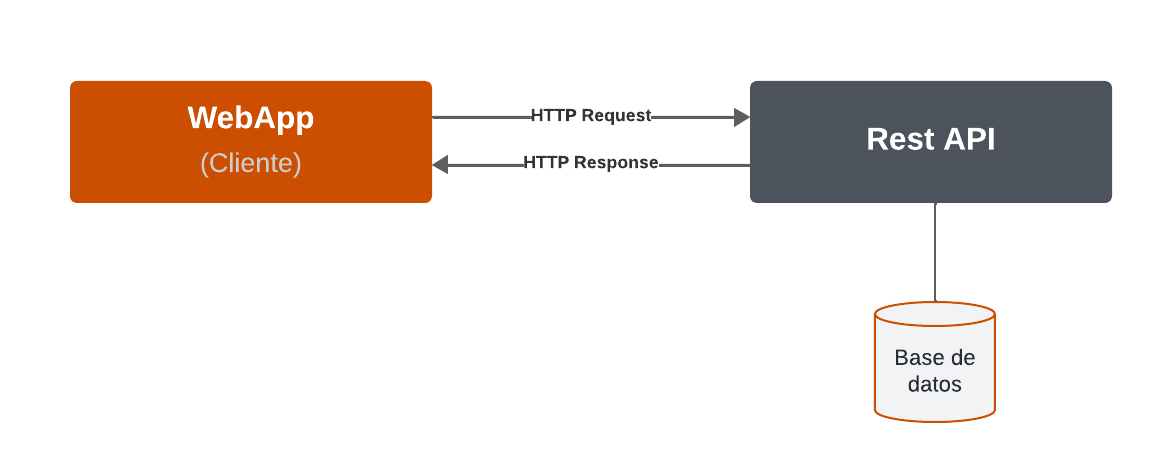
\includegraphics[width=0.7\textwidth]{figures/4-Estudio-viabilidad/4_WebApp_RestApi.png}
    \caption{Arquitectura de REST API y WebApp}
    \label{fig:arquitectura_rest_api_webapp}
    \hypertarget{fig:arquitectura_rest_api_webapp}{}
\end{figure}

\subsubsubsection{Comparativa de alternativas arquitectónicas}
Mediante la siguiente tabla, se presenta una comparación de las alternativas arquitectónicas previamente mencionadas.

\begin{table}[htb]
    \centering
    \caption{Comparación de Arquitecturas de Software}
    \label{tabla:comparacion_arquitecturas}
    \hypertarget{table:comparacion_arquitecturas}{}
    \begin{tabular}{
       >{\columncolor{rowcolor}\raggedright\arraybackslash}p{4cm}
       >{\raggedright\arraybackslash}p{3cm}
       >{\raggedright\arraybackslash}p{3cm}
       >{\raggedright\arraybackslash}p{3cm} }
    \rowcolor{lightgreen}
    \toprule
    \textbf{Criterio} & \textbf{Arquitectura Monolítica} & \textbf{Arquitectura de Microservicios} & \textbf{API REST y WebApp} \\
    \midrule
    Complejidad Inicial & Baja & Alta & Moderada \\
    \midrule
    Escalabilidad & Limitada & Alta & Moderada \\
    \midrule
    Facilidad de Mantenimiento & Alta en proyectos pequeños & Moderada a baja & Moderada si cada módulo tiene una estructura interna clara \\
    \midrule
    Despliegue & Sencillo & Complejo & Moderado \\
    \midrule
    Gestión de Proyectos & Simple en proyectos pequeños & Requiere coordinación compleja & Balanceada \\
    \midrule
    Independencia de Componentes & No & Sí & Parcial \\
    \midrule
    Adaptabilidad a Cambios & Baja & Alta & Moderada \\
    \midrule
    Recomendado para & Proyectos pequeños y simples & Proyectos grandes y escalables & Proyectos con necesidad de separación clara entre frontend y backend \\
    \bottomrule
    \end{tabular}
\end{table}


\subsubsubsection{Decisión final de la arquitectura}
Tras un análisis exhaustivo de las alternativas disponibles, se ha optado por implementar una arquitectura de API REST y WebApp.

Esta decisión permite alcanzar un equilibrio entre la simplicidad inherente a la arquitectura monolítica y la escalabilidad ofrecida por la arquitectura de microservicios. Además, esta elección facilita la gestión del proyecto mediante una separación clara entre el frontend y el backend. Tal distinción posibilita el desarrollo y despliegue independiente de cada componente, contribuyendo a la minimización de riesgos asociados a fallos en cadena. 
Además, cada módulo, operando de manera aislada, mejora significativamente la disponibilidad y confiabilidad del sistema.



\subsubsection{Valoración de alternativas para el Backend}
Es crucial seleccionar una tecnología de backend que no solo soporte eficientemente las operaciones en tiempo real sino que también se integre de manera óptima con el frontend.
A continuación, se presenta un análisis de varias alternativas para el desarrollo del backend teniendo en cuenta estos requisitos.

\subsubsubsection{Java con Spring Boot}
\coloredUnderline{\href{https://www.java.com/es/}{Java}} es un lenguaje de programación orientado a objetos que destaca por su portabilidad y robustez, siendo ampliamente utilizado en el desarrollo de aplicaciones empresariales. 
La combinación con \coloredUnderline{\href{https://spring.io/projects/spring-boot}{Spring Boot}} permite un desarrollo ágil con una amplia gama de herramientas como Spring Data y Spring Security entre otras. 
Entre sus ventajas, además de las herramientas mencionadas, destacan su escalabilidad, su robustez en el manejo de transacciones y su amplia comunidad. 
Sin embargo, Java con Spring Boot presenta una curva de aprendizaje significativa y, aunque Spring Boot puede manejar aplicaciones en tiempo real mediante Spring WebFlux, su rendimiento en este ámbito puede ser inferior comparado con otras tecnologías. Además, la integración con el frontend, podría no ser la más rápida en términos de desarrollo.

\subsubsubsection{Node.js con Express}
\coloredUnderline{\href{https://nodejs.org/es/}{Node.js}} es un entorno de ejecución para JavaScript en el lado del servidor, conocido por su modelo de I/O no bloqueante y su eficiencia en el manejo de múltiples conexiones simultáneas
La integración de Node.js con \coloredUnderline{\href{https://expressjs.com/es/}{Express}}, un framework ligero y flexible, ofrece una solución óptima para desarrollar aplicaciones web dinámicas.
Esta combinación destaca por su capacidad para gestionar operaciones en tiempo real de manera eficiente y su sinergia natural con tecnologías frontend basadas en JavaScript, facilitando un desarrollo cohesivo y ágil entre el backend y el frontend.
Como desventajas, cabe mencionar que Node.js puede no ser la opción más adecuada para tareas que requieren un alto uso de CPU debido a su naturaleza de ejecución de un solo hilo, ya que su rendimiento en este ámbito puede ser inferior al de otras tecnologías.

\subsubsubsection{Python con Django}
\coloredUnderline{\href{https://www.python.org/}{Python}}, un lenguaje de programación de alto nivel, se caracteriza por su versatilidad y amplia gama de bibliotecas. Utilizado ampliamente en 
aplicaciones empresariales combinado con \coloredUnderline{\href{https://www.djangoproject.com/}{Django}}, un framework de alto nivel que se enfoca en el desarrollo rápido y eficiente.
Como ventajas, destacan su desarrollo rápido, sus excelentes capacidades de seguridad y su buena documentación.
Aunque Django puede ser configurado para soportar aplicaciones en tiempo real mediante Django Channels, su rendimiento en estos escenarios puede no ser tan óptimo como el de Node.js. Además, aunque Django asegura una buena integración con el frontend, puede no ser la opción más ágil para aplicaciones que requieren una interacción constante.



\subsubsubsection{Comparativa de alternativas para el Backend}
En la siguiente tabla, se presenta una comparación de las alternativas para el desarrollo del Backend.
\begin{table}[H]
    \centering
    \begin{tabular}{ 
       >{\columncolor{rowcolor}\raggedright\arraybackslash}p{3cm} 
       >{\raggedright\arraybackslash}p{3cm} 
       >{\raggedright\arraybackslash}p{3cm} 
       >{\raggedright\arraybackslash}p{3cm} }
        \rowcolor{lightgreen}
    \toprule
    \textbf{Criterio} & \textbf{Java con Spring Boot} & \textbf{Node.js con Express} & \textbf{Python con Django} \\
    \midrule
    \textbf{Modelo de Programación} & Orientado a objetos, con énfasis en inyección de dependencias. & Basado en eventos y callbacks. & Orientado a componentes/modelos con énfasis en la reutilización de código. \\
    \midrule
    \textbf{Funcionalidad en tiempo real} & Buen manejo de transacciones pero menos óptimo para tiempo real. & Excelente para operaciones en tiempo real gracias a su eficiencia en I/O. & Posible pero requiere más configuración para tiempo real. \\
    \midrule
    \textbf{Integración con Frontend} & Buena, puede requerir esfuerzos adicionales. & Natural y fluida. & Buena, pero puede necesitar configuraciones extra. \\
    \midrule
    \textbf{Escalabilidad} & Alta, pero con escalabilidad vertical. & Alta, con facilidad para escalar horizontalmente. & Moderada, con algunas limitaciones en escalabilidad. \\
    \midrule
    \textbf{Seguridad} & Fuertes capacidades de seguridad. & Requiere implementaciones adicionales para seguridad. & Seguridad integrada y robusta. \\
    \bottomrule
    \end{tabular}
    \caption{Comparación de Tecnologías para el Backend}
    \label{tabla:comparacion_backend}
    \hypertarget{table:comparacion_backend}{}
    \end{table}

    
\subsubsection{Decisión final del Backend}
Considerando las necesidades del sistema a desarrollar, para soportar subastas en tiempo real y una integración fluida con el frontend la opción más adecuada es Node.js con Express.


\subsubsection{Valoración de alternativas para el Frontend}
A continuación, se presenta un análisis de alternativas para el desarrollo del frontend.

\subsubsubsection{React}
\coloredUnderline{\href{https://es.react.dev}{React}} es una biblioteca de JavaScript desarrollada y mantenida por Facebook, centrada en la construcción de interfaces de usuario a través de componentes reutilizables. Se caracteriza por su virtual DOM y su enfoque declarativo.

Entre sus ventajas, destacan su amplia comunidad, su rendimiento optimizado con Virtual DOM y su flexibilidad en la elección de estilos y componentes. 
Como desventajas cabe mencionar las actualizaciones frecuentes que implican mantenerse al día con los cambios y que necesita integración con otras herramientas para ser una solución completa.


\subsubsubsection{Angular}
\coloredUnderline{\href{https://angular.io/}{Angular}} es un framework de desarrollo web mantenido por Google, conocido por su enfoque en aplicaciones de página única (SPA). Utiliza TypeScript como lenguaje principal y proporciona un entorno robusto y completo para el desarrollo.

Entre sus ventajas, destaca su ecosistema completo, promueve un estilo de desarrollo coherente y mantenible y, además, cuenta con una comunidad activa y un amplio soporte de Google, lo que garantiza actualizaciones y soporte continuo.
Sin embargo, Angular puede ser excesivo para proyectos pequeños, ya que su curva de aprendizaje es pronunciada y su configuración inicial puede ser compleja.

\subsubsubsection{Vue.js}
\coloredUnderline{\href{https://vuejs.org/}{Vue.js}} es un framework progresivo para la construcción de interfaces de usuario, creado por Evan You. Se destaca por su facilidad de adopción, su sistema reactividad y su enfoque en la simplicidad.

Entre sus ventajas, destacan su sintaxis sencilla, su buena documentación y su facilidad de integración en proyectos existentes.
Aunque su uso va en aumento, su comunidad es más pequeña en comparación con React o Angular, lo que se traduce en menos librerías y recursos disponibles.

\subsubsubsection{Comparativa de alternativas para el Frontend}
A continuación, se presenta una comparación de las alternativas para el desarrollo del Frontend.

\begin{table}[H]
    \centering
    \begin{tabular}{ 
       >{\columncolor{rowcolor}\raggedright\arraybackslash}p{2.5cm} 
       >{\raggedright\arraybackslash}p{3.5cm} 
       >{\raggedright\arraybackslash}p{3.5cm} 
       >{\raggedright\arraybackslash}p{3.5cm} }
        \rowcolor{lightgreen}
    \toprule
    
    \textbf{Criterio} & \textbf{React} & \textbf{Angular} & \textbf{Vue.js} \\
    \midrule
    \textbf{Velocidad y Rendimiento} & Alto con Virtual DOM. Optimizado para cambios dinámicos de UI. & Buen rendimiento, pero puede ser más lento en proyectos grandes debido a su complejidad. & Rendimiento similar a React, con optimizaciones en la actualización de la UI. \\
    \midrule
    \textbf{Mantener el Estado} & Requiere bibliotecas adicionales como Redux para manejo complejo del estado. & Gestión de estado integrada, adecuada para aplicaciones complejas. & Sistema reactividad sencillo, para manejo de estado complejo requiere la biblioteca Vuex. \\
    \midrule
    \textbf{Comunidad} & Muy grande y activa, con un ecosistema extenso. & Amplia y soportada por Google, con muchas empresas adoptándolo. & Creciente y entusiasta, con un enfoque en la facilidad de uso. \\
    \midrule
    \textbf{Curva de Aprendizaje} & Moderada; JSX y el ecosistema pueden requerir tiempo de aprendizaje. & Elevada; TypeScript y su arquitectura completa requieren más tiempo para aprender. & Baja; Vue es considerado fácil de aprender, especialmente para principiantes. \\
    \midrule
    \textbf{Escalabilidad} & Muy escalable con un enfoque modular y reutilizable. & Diseñado para aplicaciones empresariales escalables y complejas. & Escalable, pero más adecuado para proyectos de tamaño mediano. \\
    \midrule
    \textbf{Ecosistemas y Módulos} & Rico ecosistema con una gran cantidad de módulos y herramientas. & Ecosistema completo con soluciones integradas para muchas necesidades. & Ecosistema más pequeño aunque en crecimiento, con módulos y librerías en aumento. \\
    \bottomrule
    \end{tabular}
    \caption{Análisis Comparativo de Frameworks y Bibliotecas de Frontend}
    \label{tabla:comparacion_frontend}
    \hypertarget{table:comparacion_frontend}{}
\end{table}

\subsubsubsection{Decisión final del Frontend}
Tras una evaluación detallada de las distintas opciones disponibles y en función de los requisitos específicos del sistema a desarrollar, se ha determinado que React es la tecnología más adecuada para el frontend.

Esta decisión se basa, principalmente, en la gran comunidad de React y en la rica colección de recursos disponles.

\subsubsection{Valoración de alternativas para la Base de Datos}
Por último, se presenta un análisis de alternativas para la base de datos del sistema.

\subsubsubsection{MySQL}
\coloredUnderline{\href{https://www.mysql.com/}{MySQL}} es un sistema de gestión de bases de datos relacional de código abierto, ampliamente utilizado en aplicaciones web. 

Entre sus ventajas, destacan su amplia adopción lo que conlleva una gran cantidad de recursos y documentación disponibles, su fiabilidad y robustez y su facilidad de uso. 

Por otro lado, MySQL puede no ser la opción más adecuada para aplicaciones que requieren de operaciones avanzadas de análisis y procesamiento de datos, ya que su rendimiento en este ámbito puede ser inferior al de otras bases de datos.

\subsubsubsection{MongoDB}
\coloredUnderline{\href{https://www.mongodb.com/}{MongoDB}} es una base de datos NoSQL orientada a documentos, diseñada para la escalabilidad y la flexibilidad. Se caracteriza por su capacidad para manejar grandes volúmenes de datos y su esquema flexible.

Entre sus ventajas, destacan su flexibilidad, permite que la base de datos crezca con la aplicación añadiendo nuevos campos a los documentos.
Además, MongoDB es altamente escalable y puede manejar grandes volúmenes de datos de manera eficiente.

Sin embargo, MongoDB puede no ser la opción más adecuada para aplicaciones que requieren transacciones ACID complejas, ya que su modelo de consistencia eventual puede no ser adecuado para todas las aplicaciones.

\subsubsubsection{PostgreSQL}
\coloredUnderline{\href{https://www.postgresql.org/}{PostgreSQL}} es un sistema de gestión de bases de datos relacional de código abierto y gratuito, conocido por su robustez, escalabilidad y soporte para transacciones ACID.

Entre sus ventajas, destacan su cumplimiento con los estándares SQL, su soporte para transacciones ACID y su capacidad para manejar grandes volúmenes de datos asegurando la integridad y seguridad de los mismos.

Como inconvenientes, cabe mencionar que PostgreSQL puede ser más lento que otras bases de datos en operaciones de lectura y escritura para bases de datos pequeñas ya que está enfocada en manejar un gran volumen de datos,
 y su curva de aprendizaje puede ser pronunciada para usuarios no familiarizados con SQL.

\subsubsubsection{Comparativa de alternativas para la Base de Datos}
En la siguiente tabla, se presenta una comparación de las alternativas para la base de datos del sistema.
\begin{table}[H]
    \centering
    \begin{tabular}{ 
       >{\columncolor{rowcolor}\raggedright\arraybackslash}p{3cm} 
       >{\raggedright\arraybackslash}p{3cm} 
       >{\raggedright\arraybackslash}p{3cm} 
       >{\raggedright\arraybackslash}p{3cm} }
        \rowcolor{lightgreen}
    \toprule
    \textbf{Criterio} & \textbf{MySQL} & \textbf{MongoDB} & \textbf{PostgreSQL} \\
    \midrule
    \textbf{Tipo de Base de Datos} & Relacional & NoSQL & Relacional \\
    \midrule
    \textbf{Modelo de Datos} & Tablas y Filas & Documentos JSON/BSON & Tablas y Filas \\
    \midrule
    \textbf{Lenguaje de Consulta} & SQL & MongoDB Query Language (MQL) & SQL \\
    \midrule
    \textbf{Escalabilidad} & Escalabilidad vertical y soporte para horizontal & Escalabilidad horizontal mediante sharding & Escalabilidad vertical y horizontal \\
    \midrule
    \textbf{Transacciones} & Soporte completo de ACID & Soporte parcial de ACID en ciertas operaciones & Soporte completo de ACID \\
    \midrule
    \textbf{JSON} & Soporte limitado mediante campos JSON & JSON nativo & Soporte avanzado de JSON y JSONB \\
    \midrule
    \textbf{Flexibilidad de Esquema} & Esquemas rígidos & Esquemas flexibles& Esquemas rígidos \\
    \midrule
    \textbf{Rendimiento} & Alto rendimiento en lecturas & Alto rendimiento en escrituras & Alto rendimiento en lecturas y escrituras \\
    \bottomrule
    \end{tabular}
    \caption{Comparativa entre MySQL, MongoDB y PostgreSQL}
    \label{tabla:comparacion_bases_datos}
    \hypertarget{table:comparacion_bases_datos}{}
\end{table}


\subsubsection{Decisión final de la Base de Datos}
Tras un análisis detallado de las distintas opciones disponibles y en función de los requisitos específicos del sistema a desarrollar, se ha determinado que MongoDB es la tecnología más adecuada para la base de datos. 

Esta elección se basa en un \textit{trade-off}, es decir, se acepta la falta de integridad referencial y la consistencia eventual a cambio de una mayor flexibilidad y escalabilidad en el manejo de datos que es lo que se necesita para el sistema a desarrollar.

De esta manera, con todas decisiones anteriores se obtiene una arquitectura MERN (MongoDB, Express, React, Node.js), ejemplificada en la \coloredUnderline{\hyperlink{fig:arquitectura_mern}{Figura \ref*{fig:arquitectura_mern}: \nameref*{fig:arquitectura_mern}}},comunmente utilizada en aplicaciones web modernas y que se ajusta a las necesidades del proyecto. 
Se puede consultar más información sobre la arquitectura MERN en el siguiente enlace: \coloredUnderline{\href{https://www.mongodb.com/resources/languages/mern-stack}{MERN Stack}}.
\begin{figure}[H]
    \centering
    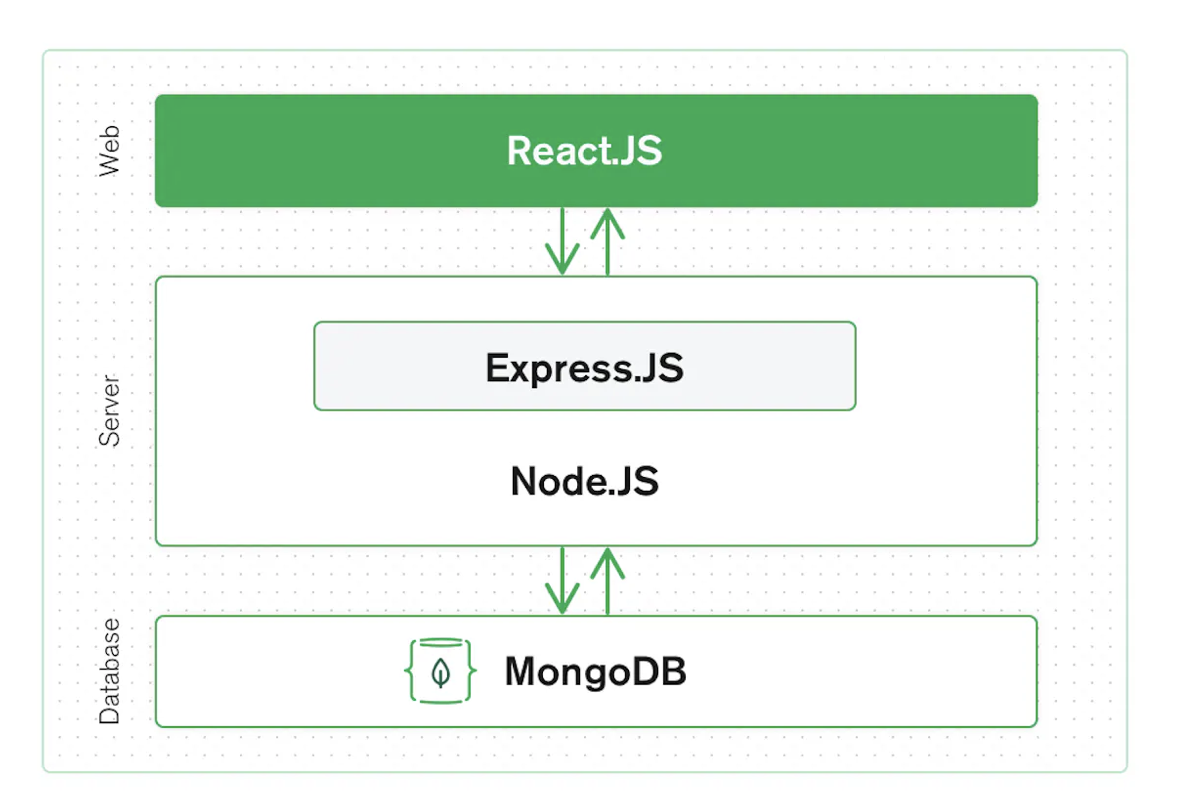
\includegraphics[width=0.5\textwidth]{figures/4-Estudio-viabilidad/4_MERN.png}
    \caption{MERN Stack: MongoDB, Express, React, Node.js}
    \label{fig:arquitectura_mern}
    \hypertarget{fig:arquitectura_mern}{}
\end{figure}
